\documentclass[a4paper,11pt]{article}

\usepackage[utf8]{inputenc}
\usepackage[T1]{fontenc}
\usepackage[spanish]{babel}
\usepackage{geometry}
\usepackage{graphicx}
\usepackage{subcaption}
\usepackage{booktabs}
\usepackage{float}
\usepackage{amsmath}
\usepackage{hyperref}
\usepackage{xcolor}

\geometry{margin=2.5cm}
\hypersetup{
    colorlinks=true,
    linkcolor=blue!50!black,
    urlcolor=blue!50!black,
    citecolor=blue!50!black
}

\title{Informe de ejercicios de Visión por Computador}
\author{}
\date{}

\begin{document}

\maketitle

\section{Resumen general}

Este informe resume los cuatro ejercicios desarrollados: Wide ResNet sobre CIFAR-10, reconocimiento de género con CNNs, segmentación de lesiones ISIC con U-Net y visualización de mapas de atención en Vision Transformers. El objetivo no es solo listar métricas, sino relacionarlas con lo que pedía el enunciado y valorar hasta qué punto los resultados son convincentes.

\begin{table}[H]
\centering
\begin{tabular}{p{0.24\linewidth} p{0.34\linewidth} p{0.34\linewidth}}
\toprule
\textbf{Ejercicio} & \textbf{Petición del enunciado} & \textbf{Resultado obtenido} \\
\midrule
Wide ResNet en CIFAR-10 & Implementar una topología avanzada tipo Wide ResNet. & WRN-16-4 con aumento de datos; \(91.95\%\) de accuracy en test. \\
Reconocimiento de género & Un modelo \(>98\%\) y otro \(>95\%\) con menos de 100K parámetros. & Modelo pequeño: \(95.35\%\) con 64,466 parámetros entrenables. Modelo fuerte: \(97.62\%\), cerca del objetivo de \(98\%\) pero por debajo. \\
Segmentación ISIC & Implementar U-Net, dividir 80/20 y evaluar sobre test. & 2,750 pares imagen-máscara; test de 550 imágenes; Dice \(0.8663\), IoU \(0.7642\). \\
Atención en ViT & Extraer y visualizar mapas de atención de varias capas. & ViT tiny preentrenado, capas 0, 3, 6 y 11, media de cabezas y attention rollout en cuatro imágenes. \\
\bottomrule
\end{tabular}
\caption{Resumen de los ejercicios realizados y su relación con los objetivos.}
\end{table}

\section{Wide ResNet sobre CIFAR-10}

\subsection{Objetivo y configuración}

El enunciado pedía trabajar con topologías avanzadas, en concreto Wide ResNet. La implementación usada es una WRN-16-4: profundidad 16, factor de ensanchamiento 4 y dos bloques residuales por etapa. La entrada es la imagen CIFAR-10 de \(32\times32\times3\). Tras una convolución inicial de 16 filtros, el modelo pasa por tres etapas residuales con 64, 128 y 256 canales; las dos últimas reducen la resolución espacial a \(16\times16\) y \(8\times8\). Finalmente se aplica \textit{global average pooling} y una capa densa de 10 clases.

El entrenamiento se hizo con aumento de datos mediante padding, recorte aleatorio y volteo horizontal. Esto es importante en CIFAR-10 porque el conjunto es pequeño para un modelo de 2.75 millones de parámetros, y sin regularización el riesgo de sobreajuste sería alto.

\begin{table}[H]
\centering
\begin{tabular}{lr}
\toprule
\textbf{Métrica} & \textbf{Valor} \\
\midrule
Parámetros totales & 2,754,298 \\
Imágenes de entrenamiento & 45,000 \\
Imágenes de validación & 5,000 \\
Imágenes de test & 10,000 \\
Mejor accuracy de validación & \(92.62\%\) \\
Accuracy de test & \(91.95\%\) \\
Loss de test & 0.4778 \\
\bottomrule
\end{tabular}
\caption{Resultados principales de la WRN-16-4 en CIFAR-10.}
\end{table}

\begin{figure}[H]
\centering
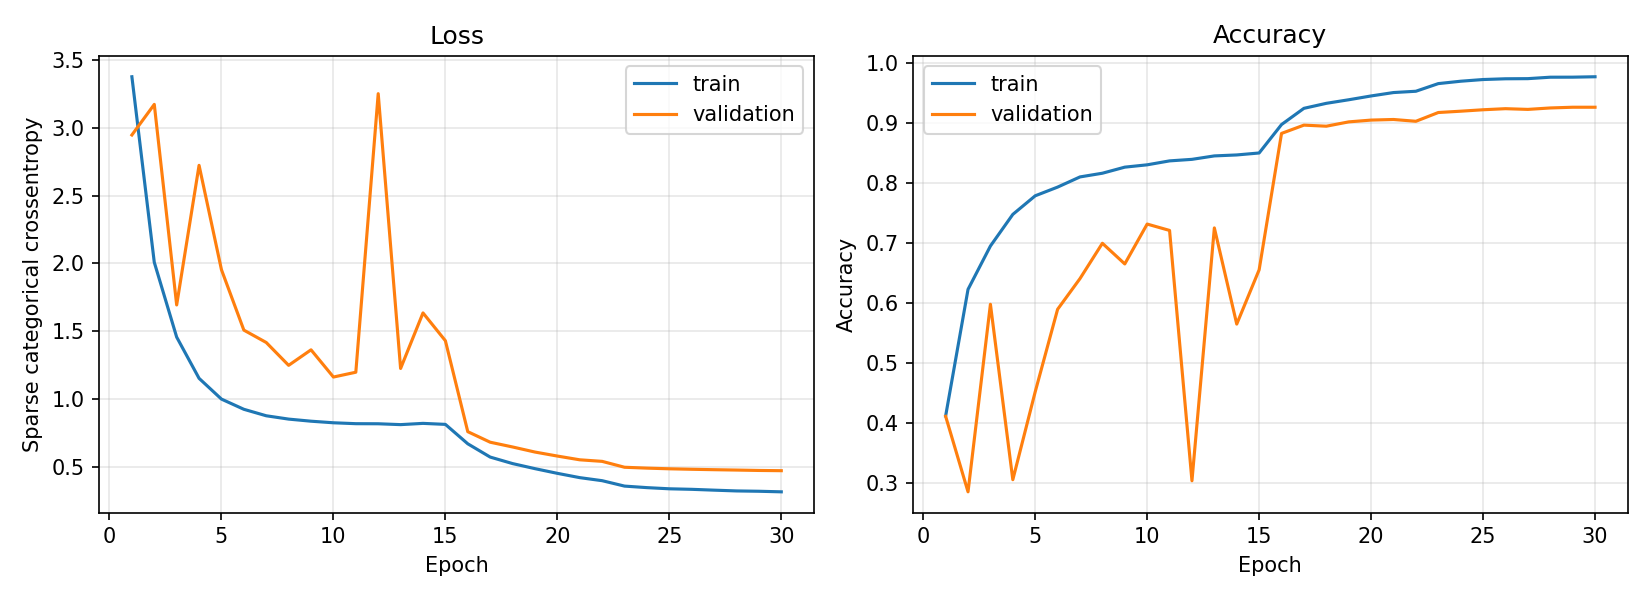
\includegraphics[width=0.95\linewidth]{results_cifar_wrn/training_curves.png}
\caption{Curvas de entrenamiento de la Wide ResNet.}
\end{figure}

\begin{figure}[H]
\centering
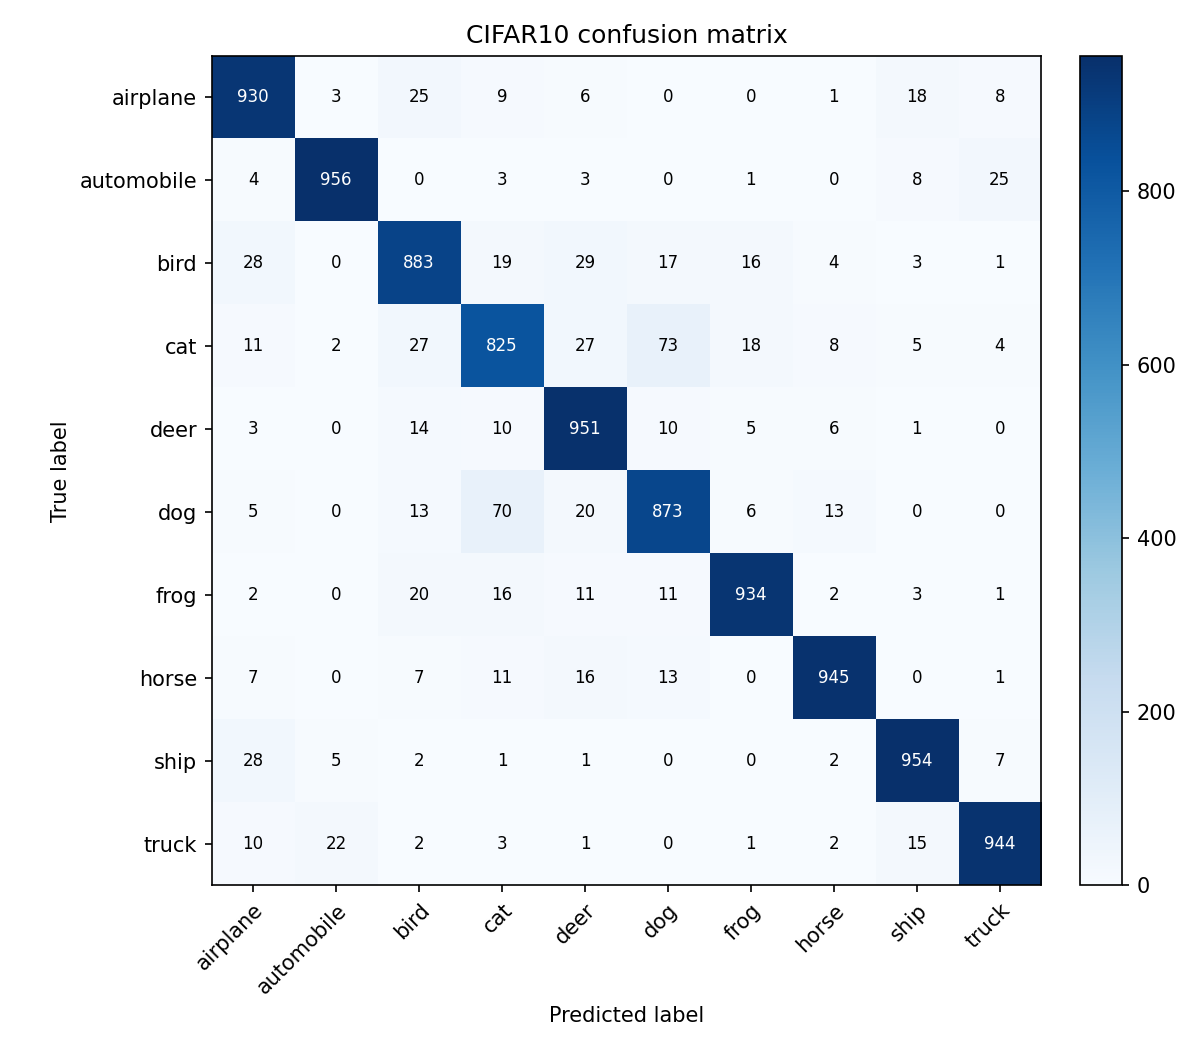
\includegraphics[width=0.72\linewidth]{results_cifar_wrn/confusion_matrix.png}
\caption{Matriz de confusión en CIFAR-10.}
\end{figure}

\subsection{Comentario}

El resultado es bueno para una implementación entrenada desde cero en CIFAR-10: el \(91.95\%\) en test indica que la red aprende representaciones robustas y que el ensanchamiento de los bloques residuales funciona bien. La diferencia entre validación y test es pequeña, por lo que no parece haber una brecha grave de generalización.

La matriz de confusión muestra los errores esperables del dataset. Las clases con más confusión son \textit{cat} y \textit{dog}: por ejemplo, 73 gatos se predicen como perros y 70 perros como gatos. También hay confusiones moderadas entre \textit{automobile} y \textit{truck}. Esto tiene sentido porque son categorías visualmente próximas y con variabilidad de pose y fondo. En cambio, clases como \textit{automobile}, \textit{ship}, \textit{horse} y \textit{deer} quedan bastante bien separadas.

\section{Reconocimiento de género}

\subsection{Objetivo y modelos}

El ejercicio de reconocimiento de género planteaba dos metas: superar el \(98\%\) de accuracy en test y construir otro modelo que superase el \(95\%\) con menos de 100K parámetros. Se entrenaron dos CNNs sobre las imágenes LFW recortadas a \(100\times100\) RGB:

\begin{itemize}
    \item \textbf{Modelo pequeño}: usa convoluciones separables, normalización por lotes, \textit{dropout} y \textit{global average pooling}. Su diseño está claramente orientado a cumplir la restricción de tamaño.
    \item \textbf{Modelo fuerte}: usa bloques de dos convoluciones estándar, max pooling progresivo, más canales y una capa densa final mayor.
\end{itemize}

Ambos modelos usaron aumento ligero de datos: volteo horizontal, rotaciones pequeñas, traslaciones y zoom. La distribución de test está desbalanceada: 2,052 ejemplos de la clase 0 frente a 596 de la clase 1, así que conviene mirar también precisión, recall y F1, no solo accuracy.

\begin{table}[H]
\centering
\begin{tabular}{lrrrr}
\toprule
\textbf{Modelo} & \textbf{Parámetros entrenables} & \textbf{Accuracy test} & \textbf{Loss test} & \textbf{F1 clase 1} \\
\midrule
Pequeño & 64,466 & \(95.35\%\) & 0.1229 & 0.8957 \\
Fuerte & 2,158,306 & \(97.62\%\) & 0.0739 & 0.9466 \\
\bottomrule
\end{tabular}
\caption{Comparación de los dos modelos de reconocimiento de género.}
\end{table}

\begin{figure}[H]
\centering
\begin{subfigure}{0.49\linewidth}
    \centering
    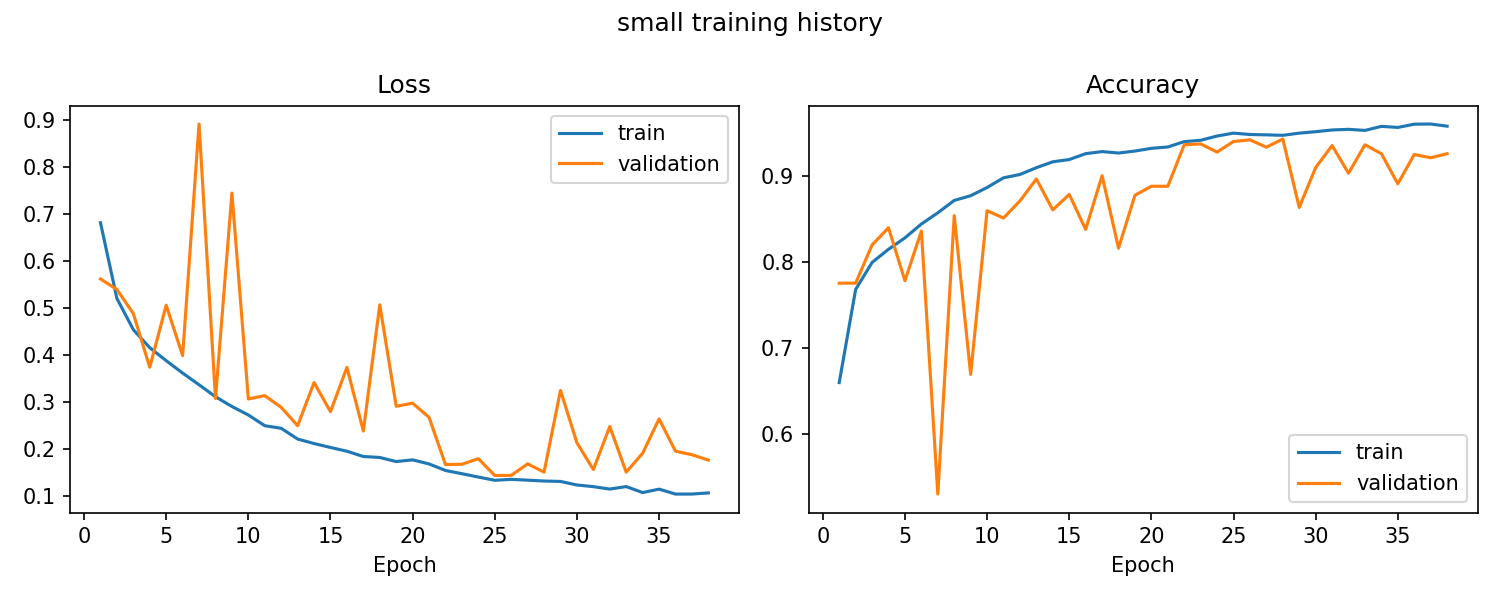
\includegraphics[width=\linewidth]{results_gender/history_small.png}
    \caption{Modelo pequeño.}
\end{subfigure}
\hfill
\begin{subfigure}{0.49\linewidth}
    \centering
    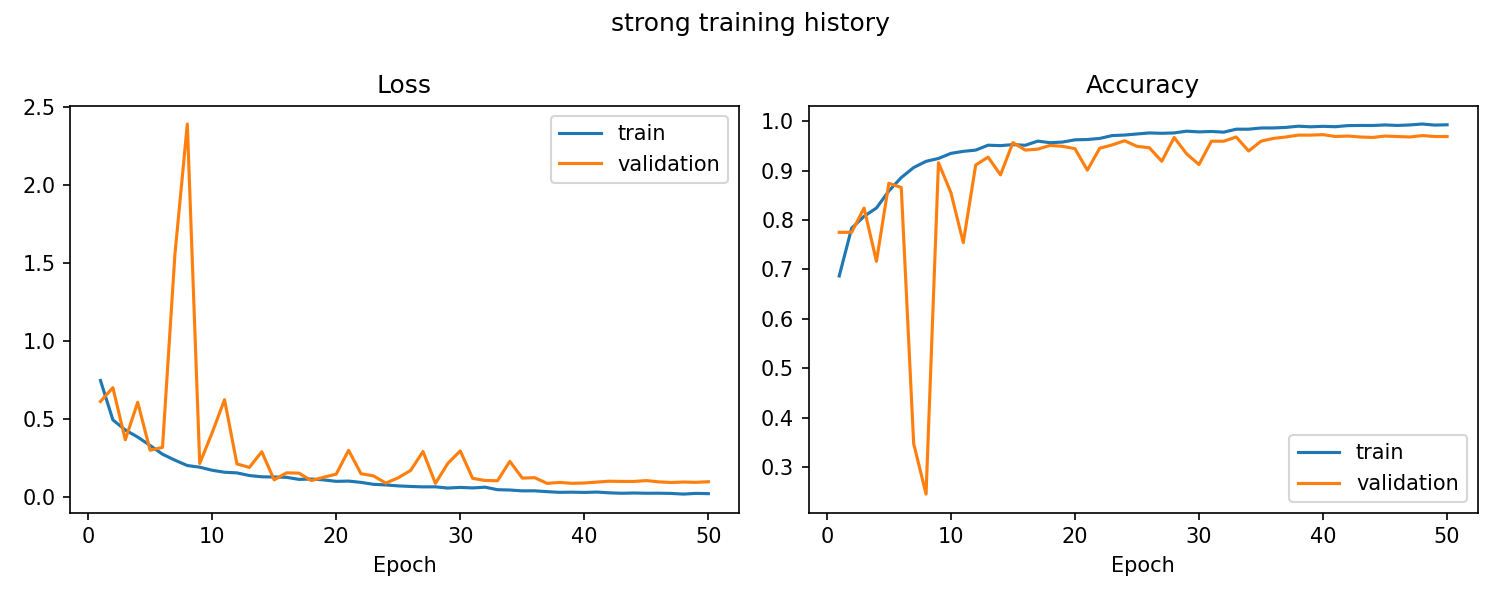
\includegraphics[width=\linewidth]{results_gender/history_strong.png}
    \caption{Modelo fuerte.}
\end{subfigure}
\caption{Curvas de entrenamiento y validación para reconocimiento de género.}
\end{figure}

\begin{figure}[H]
\centering
\begin{subfigure}{0.47\linewidth}
    \centering
    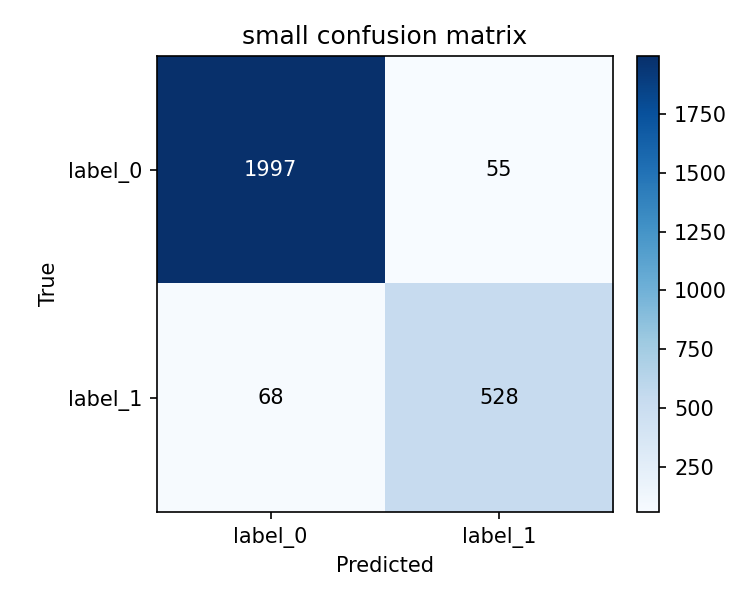
\includegraphics[width=\linewidth]{results_gender/confusion_matrix_small.png}
    \caption{Modelo pequeño.}
\end{subfigure}
\hfill
\begin{subfigure}{0.47\linewidth}
    \centering
    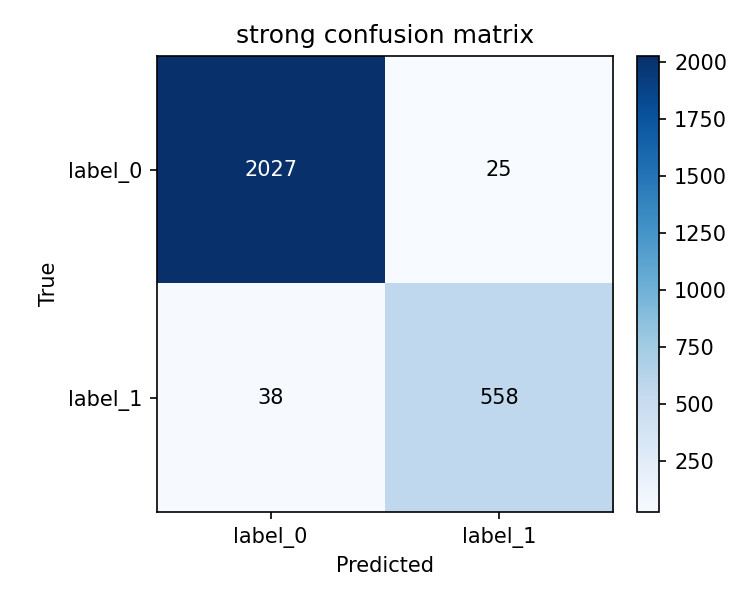
\includegraphics[width=\linewidth]{results_gender/confusion_matrix_strong.png}
    \caption{Modelo fuerte.}
\end{subfigure}
\caption{Matrices de confusión en el conjunto de test.}
\end{figure}

\subsection{Comentario}

El modelo pequeño cumple exactamente la parte más interesante de la práctica: supera el \(95\%\) usando solo 64,466 parámetros entrenables. Esto sugiere que, para este problema, una arquitectura eficiente con convoluciones separables es suficiente para capturar buena parte de la señal visual. Aun así, el F1 de la clase minoritaria es \(0.8957\), claramente inferior al de la clase mayoritaria. No es un fallo sorprendente: el desbalance del conjunto hace que el modelo tenga menos ejemplos de esa clase y el recall baja a \(0.8859\).

El modelo fuerte mejora bastante la clasificación de la clase minoritaria: su F1 sube a \(0.9466\) y el accuracy global alcanza \(97.62\%\). Sin embargo, no llega al \(98\%\) pedido por el enunciado. La diferencia es pequeña, pero conviene ser honesto: el objetivo principal de máxima accuracy queda cerca, no completamente cumplido. Para intentar cerrar esa brecha podrían probarse más épocas con parada temprana, reponderación de clases, un ajuste más fino del learning rate o un modelo preentrenado ligero.

\section{Segmentación ISIC con U-Net}

\subsection{Objetivo y configuración}

El ejercicio pedía implementar una U-Net para segmentación binaria de lesiones de melanoma, dividir los datos en 80\% entrenamiento y 20\% test y reportar resultados sobre test. El conjunto usado contiene 2,750 pares imagen-máscara. La división final reserva 550 imágenes para test; del 80\% restante se apartan 220 imágenes para validación, por lo que el entrenamiento efectivo usa 1,980 imágenes.

La red implementada es una U-Net clásica con bloques \textit{DoubleConv}: dos convoluciones \(3\times3\), batch normalization y ReLU. El encoder usa max pooling y duplica canales progresivamente; el decoder usa convoluciones transpuestas y conexiones de salto con las activaciones del encoder. La función de pérdida combina BCEWithLogitsLoss con pérdida Dice, una decisión razonable porque la segmentación de lesiones suele tener desbalance fuerte entre fondo y lesión.

\begin{table}[H]
\centering
\begin{tabular}{lr}
\toprule
\textbf{Métrica en test} & \textbf{Valor} \\
\midrule
Loss & 0.3328 \\
Dice & 0.8663 \\
IoU & 0.7642 \\
Pixel accuracy & \(94.70\%\) \\
Mejor época & 29 \\
Mejor Dice de validación & 0.8723 \\
\bottomrule
\end{tabular}
\caption{Resultados de segmentación ISIC.}
\end{table}

\begin{figure}[H]
\centering
\begin{subfigure}{0.49\linewidth}
    \centering
    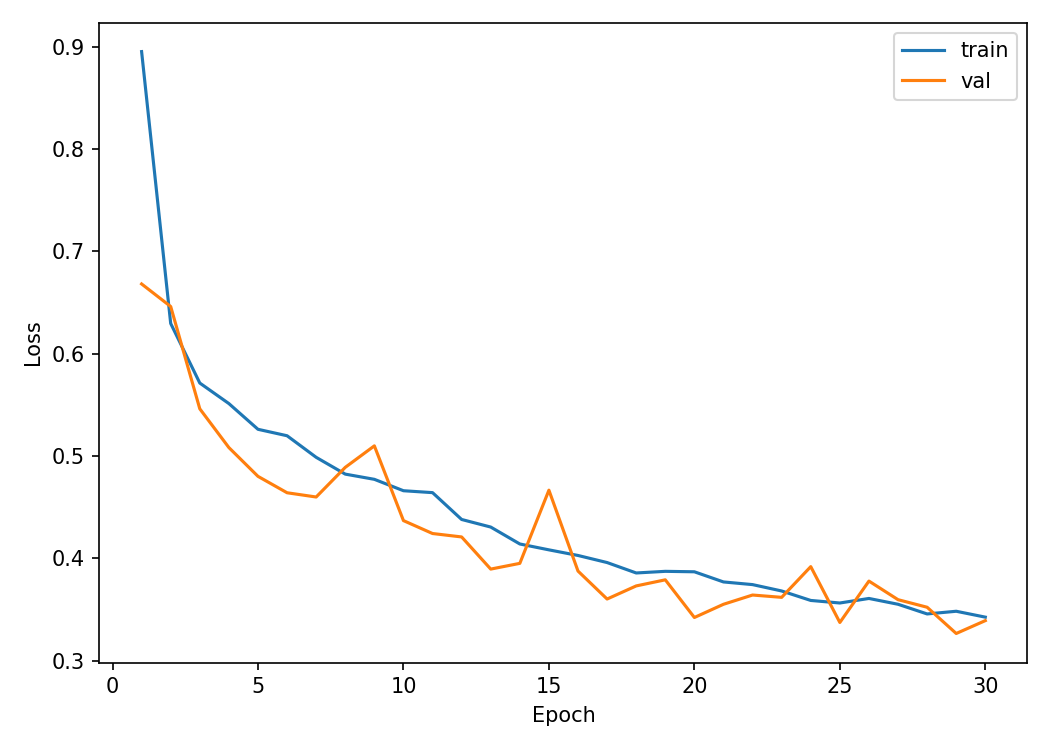
\includegraphics[width=\linewidth]{results_isic_unet/loss_curve.png}
    \caption{Loss.}
\end{subfigure}
\hfill
\begin{subfigure}{0.49\linewidth}
    \centering
    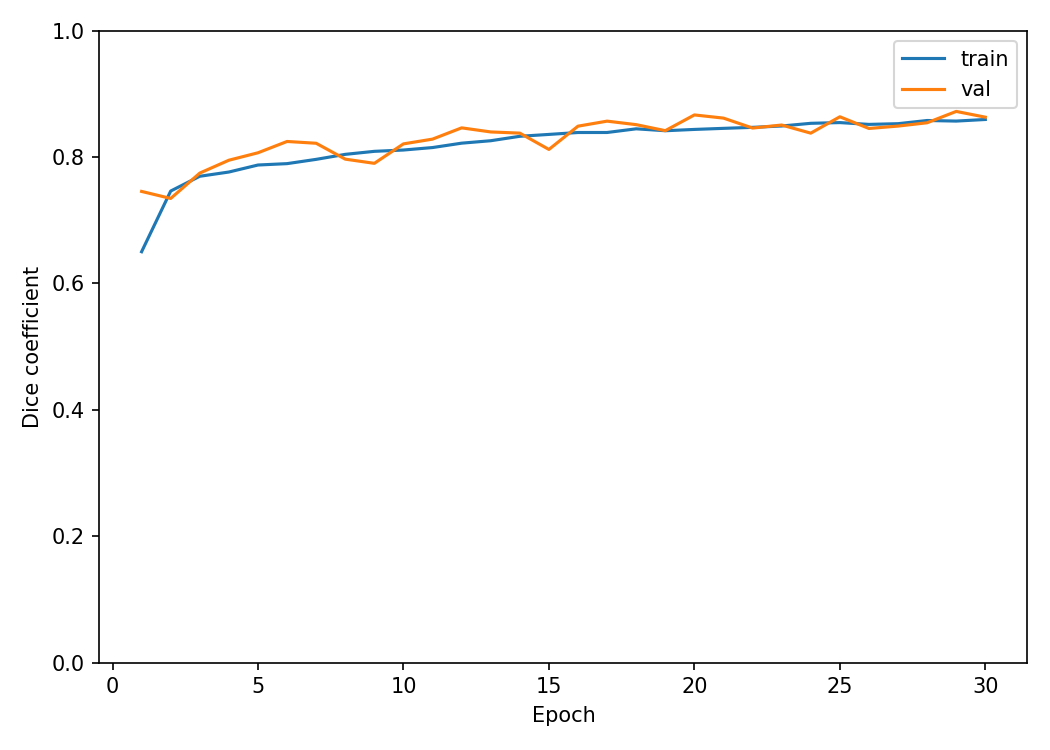
\includegraphics[width=\linewidth]{results_isic_unet/dice_curve.png}
    \caption{Dice.}
\end{subfigure}
\caption{Evolución del entrenamiento de la U-Net.}
\end{figure}

\begin{figure}[H]
\centering
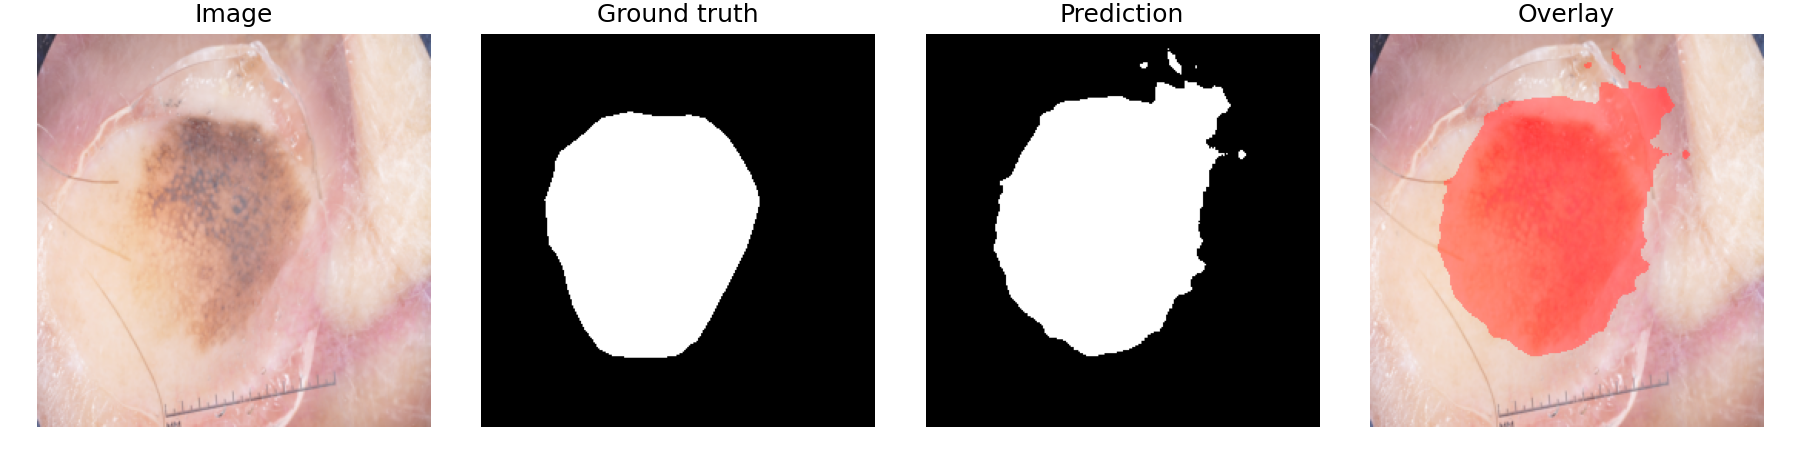
\includegraphics[width=0.98\linewidth]{results_isic_unet/examples/example_000.png}
\caption{Ejemplo cualitativo de segmentación: imagen, máscara real, predicción y superposición.}
\end{figure}

\subsection{Comentario}

El Dice de \(0.8663\) y el IoU de \(0.7642\) son resultados sólidos para una U-Net entrenada de forma directa en CPU y con imágenes redimensionadas a \(256\times256\). La pixel accuracy de \(94.70\%\) es positiva, pero en segmentación médica no debe interpretarse sola: si el fondo ocupa mucha superficie, una accuracy alta puede esconder errores en el contorno de la lesión. Por eso Dice e IoU son métricas más informativas.

La curva de validación alcanza su mejor Dice en la época 29, prácticamente al final del entrenamiento. Esto sugiere que el modelo todavía estaba aprovechando las últimas épocas y que no hay una señal clara de sobreajuste severo. Los ejemplos cualitativos son importantes porque permiten ver si los errores son pequeños desplazamientos de borde, huecos internos o fallos grandes de localización; en una aplicación médica, ese análisis visual es tan relevante como la tabla de métricas.

\section{Visualización de atención en Vision Transformers}

\subsection{Objetivo y configuración}

El objetivo del ejercicio era extraer mapas de atención de un ViT preentrenado, proyectarlos sobre imágenes y comparar distintas capas. Se usó \texttt{vit\_tiny\_patch16\_224} de \texttt{timm}, con mapas de las capas 0, 3, 6 y 11. Para cada capa se promedió la atención entre cabezas, y además se generó \textit{attention rollout}, que acumula la propagación de atención a través de todos los bloques.

La extracción se hizo mediante \textit{hooks} sobre los módulos de atención del modelo. También se desactivó la atención fusionada para que los tensores de atención fueran accesibles. Se procesaron cuatro imágenes: una imagen ISIC, su máscara de segmentación, una imagen de coches y una imagen CIFAR-10.

\begin{table}[H]
\centering
\begin{tabular}{lrr}
\toprule
\textbf{Imagen} & \textbf{Clase top-1 ImageNet} & \textbf{Confianza} \\
\midrule
ISIC\_0000000.jpg & 78 & 0.4123 \\
ISIC\_0000000\_segmentation.png & 633 & 0.0644 \\
cars.png & 609 & 0.7912 \\
cifar10.png & 916 & 0.3964 \\
\bottomrule
\end{tabular}
\caption{Predicciones del ViT preentrenado para las imágenes usadas en la visualización.}
\end{table}

\begin{figure}[H]
\centering
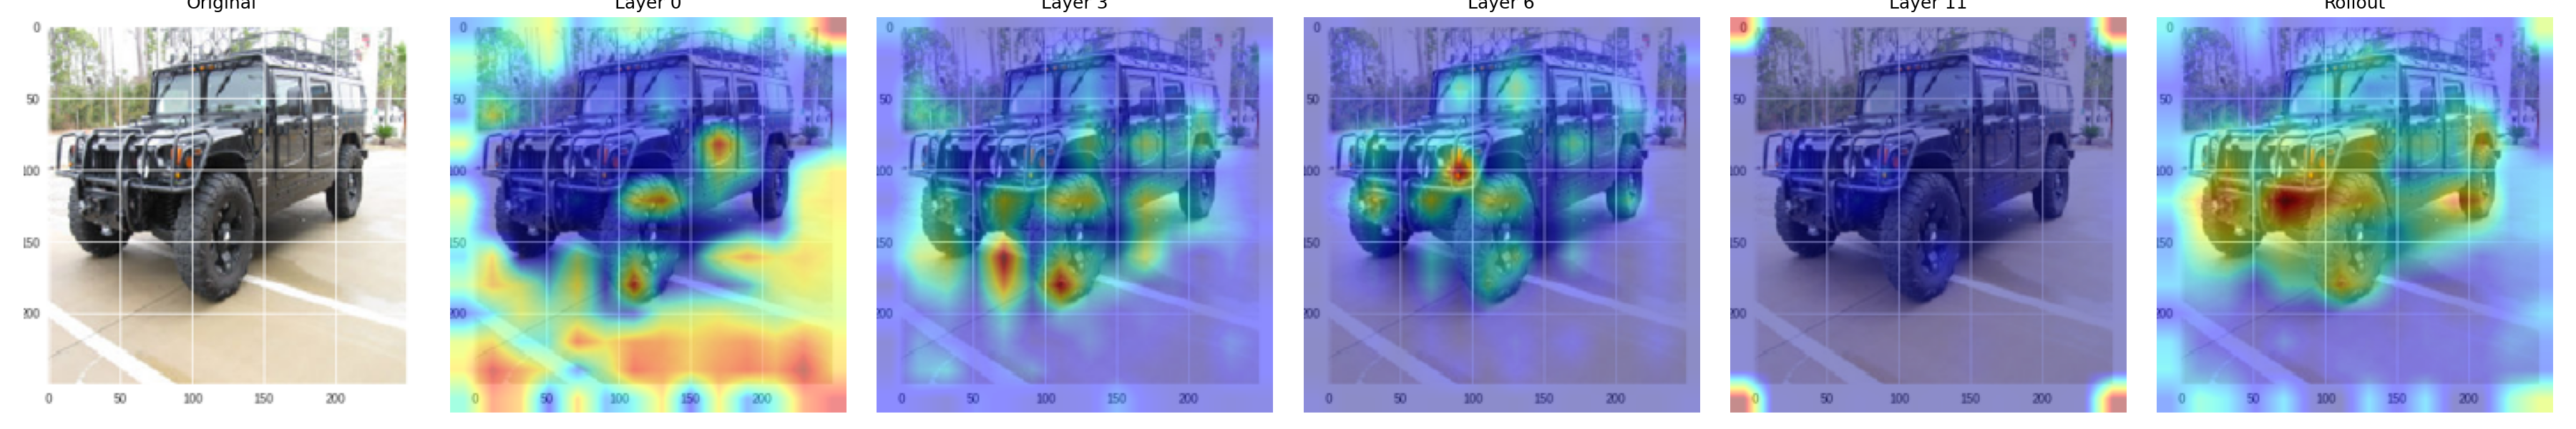
\includegraphics[width=\linewidth]{results_vit_attention/cars/attention_grid.png}
\caption{Comparación de mapas de atención por capas y rollout para la imagen de coches.}
\end{figure}

\begin{figure}[H]
\centering
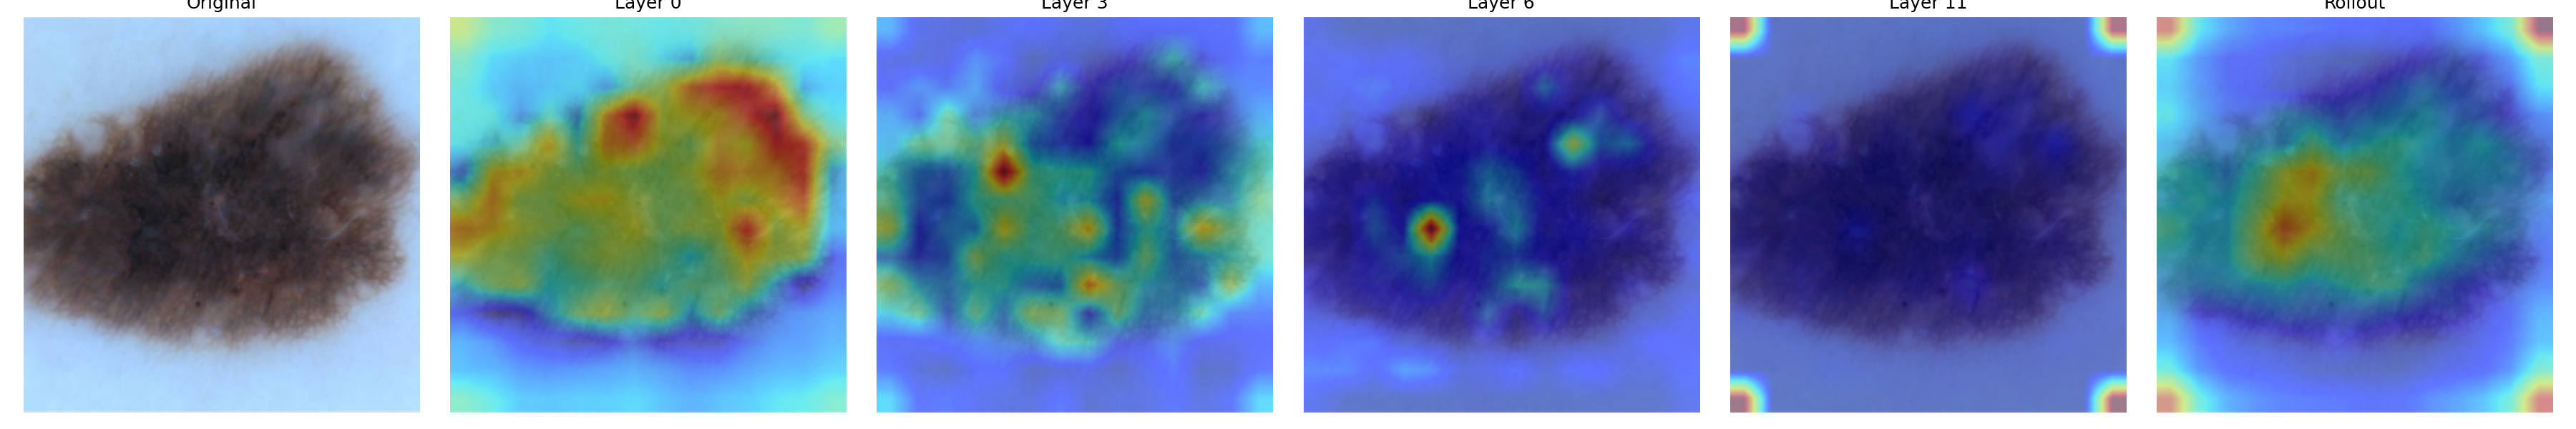
\includegraphics[width=\linewidth]{results_vit_attention/ISIC_0000000/attention_grid.png}
\caption{Comparación de mapas de atención por capas y rollout para la imagen ISIC.}
\end{figure}

\subsection{Comentario}

La comparación entre capas es coherente con el comportamiento habitual de los ViT. Las capas iniciales tienden a atender a patrones locales, bordes y texturas; las capas intermedias empiezan a agrupar regiones más amplias; y las capas finales concentran más la atención en zonas semánticamente relevantes para la predicción. El attention rollout produce mapas más suaves y globales, por lo que resulta útil para interpretar la acumulación de información, aunque pierde detalle fino frente a una capa concreta.

La imagen de coches tiene una confianza alta (\(0.7912\)), lo cual tiene sentido porque pertenece a un dominio cercano a ImageNet. En cambio, la máscara de segmentación ISIC tiene confianza muy baja (\(0.0644\)): es una imagen artificial, fuera del dominio natural de entrenamiento del ViT. Este resultado es útil porque recuerda una limitación importante de los mapas de atención: visualizan qué usa el modelo, pero no garantizan que la predicción sea correcta ni clínicamente significativa. Para imágenes médicas, un ViT preentrenado en ImageNet puede producir mapas visualmente razonables sin estar realmente especializado en la tarea.

\section{Conclusiones}

Los resultados cubren bien cuatro partes del enunciado. La Wide ResNet demuestra una topología avanzada con buen rendimiento en CIFAR-10. En reconocimiento de género, el modelo compacto cumple el objetivo de menos de 100K parámetros y más del \(95\%\), mientras que el modelo grande queda cerca pero no alcanza el \(98\%\). En segmentación, la U-Net obtiene métricas consistentes y razonables, especialmente en Dice. Finalmente, el ejercicio de ViT cumple la parte cualitativa de extracción y comparación de atención, incluyendo rollout.

Como valoración global, los experimentos están bien orientados: no se limitan a entrenar modelos, sino que guardan curvas, matrices de confusión, informes de clasificación, ejemplos cualitativos y mapas de atención. La principal mejora pendiente sería profundizar en el ajuste de hiperparámetros del modelo fuerte de género y, si se quisiera ampliar el informe, añadir una comparación cuantitativa CNN vs Transformer para clasificación, que es otro de los apartados avanzados del enunciado.

\end{document}
